\chapter{Formative Studies}
\label{sec:formative}

% TODO: need a paragraph here to explain the tiny ethnography: why I
% did it, why it is relevant

The previous chapter covered background literature and prior work
carried out by other researchers. In this chapter, I present original
work studying design culture, specifically related to rapid
fabrication with laser cutters.

There are three studies. First, I give observations of people working
at a professional design studio. This gives a firsthand account of the
processes that real designers use when practicing their craft. Second,
to better understand the tasks and problems designers face when
designing for laser cutters, we conducted two related formative
studies.  In the first, we interviewed people with experience
designing these artifacts and watched them work. In the second, we
surveyed and analyzed laser-cut items found on community web sites to
identify common features.

\section{Tiny Ethnography}
\label{sec:formative-tiny-ethnography}

% TODO: this entire section was copied from my workshop paper. Edit it
% to make it serve the larger point.
I arranged to ``be a fly on the wall'' at a well-respected design firm
in the Pittsburgh area to observe how designers work. I spent about
twenty hours at the company observing and interviewing the designers
who work there. This study was inspired by Bucciarelli's ethnographies
of engineers~\cite{bucciarelli-designing-engineers}. While this work
pre-dates my focus on design for laser cutters, it does provide a
solid connection between my narrow topic and the broader context of
design practice.

A professional studio is notably different than an educational design
studio. For example, many issues companies face are generally not
present in an academic institution. These include billable hours,
interacting with paying customers, significant differences in age and
experience level of collaborators, and so on. 

This company's culture places high value on collaborative whiteboard
sessions. At any time, the majority whiteboard surfaces throughout the
office have some sort of scribbling on them. Most whiteboard sessions
were made as two or more people gathered in conversation. The
 scribbles served to represent objects that are sometimes
labeled with markers, but usually just described verbally. In this
way, collaborative whiteboard sessions are multi-modal design
artifacts, because part of their value is static (scribbles on the
whiteboard), while another part is transient (the conversation at the
time of the scribbling)~\cite{ju-navigator}. These whiteboard sessions
are consistent with Ferguson's \textit{talking
  sketches}~\cite{ferguson-engineering}.

Four of the five designers I interviewed showed me their paper
sketches. About half of these drawings were made when the designer was
alone (Ferguson's \textit{thinking sketch}), and the rest resulted
from collaborative sessions like the whiteboard events described
above. Some paper sketches were diagrammatic (using formal or
semi-formal notation), while others were renderings of some physical
object like a building or electronic gadget. Interestingly, those same
designers were less inclined to show computational models like
Illustrator files because they felt the sketches contained the
``real'' work.

While designers did not typically voluntarily show computational
artifacts, they were inclined to show me printed versions of their
computational models. Nearly all of these printed pages had
handwriting and sketches on them, sometimes by more than one
person. People reported that they use a process of iterating between
virtual and paper versions of their designs. The designers would edit
a computational model with a high functionality application such as
Photoshop, and then print a paper copy for personal or group use. They
would then draw or write directly on that page as they explored
variations or made refinements. If a paper-based editing session was
useful, the designers would then manually transfer these changes back
into their application. The process of printing, editing, and manually
merging changes was seen repeatedly. This pattern recurs in the
following section on laser cutter users.

\section{Interviews}
\label{sec:formative-interviews}

\begin{figure}[t]
  \centering
  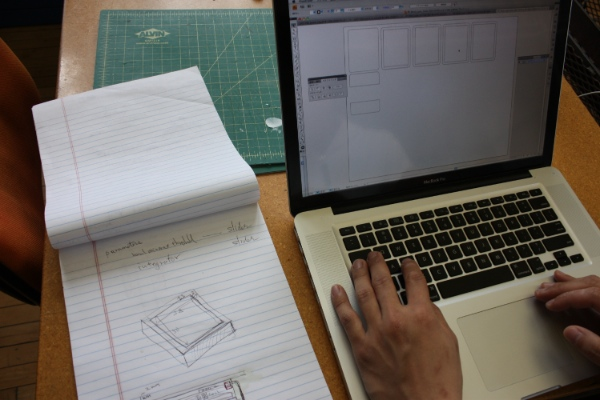
\includegraphics[width=0.7\linewidth]{img/translate-sketch-to-computer.jpg}
  \caption[Translating paper sketch to computer model]{A common step
    of designing for laser cutters: translating a hand-made sketch to
    a computer modeling tool. The sketch includes a perspective
    drawing of the desired result, and 2D diagrams of individual parts
    with key dimensions indicated.}
  \label{fig:translate}
\end{figure}


I interviewed six designers from different backgrounds, including
mechanical engineering, graphic design, and architecture to learn
about their work practices and to understand how they use their
tools. All were experienced with designing objects to be made with a
laser cutter.

Each session lasted approximately one hour, split evenly between an
interview and using software. We met participants in their workplaces,
and asked them to describe their design process and to show sketches
or videos of their work. Although there were differences in their
process, each followed the same overall pattern.

The designers all said they began by thinking about a problem and
sketching on paper. They made drawings to think about how to ``frame''
the project (what it is for). Other sketches helped reason about how
to make it (how it works and fits together). Some designers explicitly
noted that sketching is a necessary part of the process: they could
not move forward without making freehand drawings. Only after the idea
is well-formed were they ready to translate their hand-made sketch
into a computer model (Figure~\ref{fig:translate}).

After the interview, we asked participants to copy the sketch shown in
Figure~\ref{fig:interview-sketch} using a software tool of their
choice. We wanted to learn what problems people encountered when
executing the common task of translating a sketch to a computer model.


\begin{figure}[t]
\centering \subfloat[We asked users to replicate this sketched part.]
           {
  \label{fig:interview-sketch-1} 
  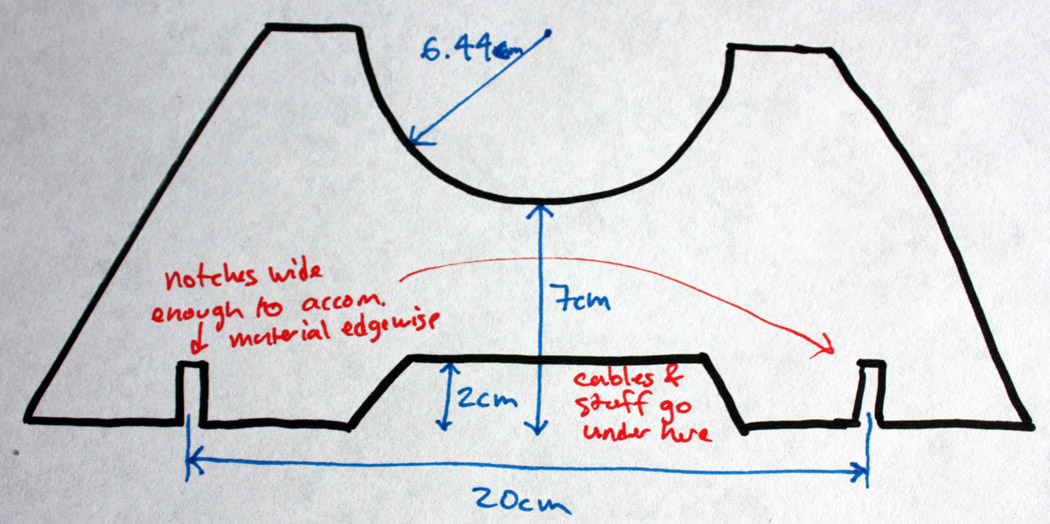
\includegraphics[width=0.7\linewidth]{img/laser-me-1.jpg}
}

\subfloat[Drawing of the part in context.] {
    \label{fig:interview-sketch-2}
    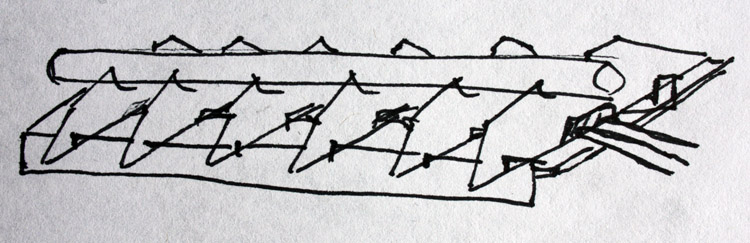
\includegraphics[width=0.7\linewidth]{img/laser-me-2.jpg}
}
\caption[Sketch from designer interview activity]{We asked
  participants to model the part at the top using a software of their
  choice.}
\label{fig:interview-sketch}
\end{figure}


Five participants chose to implement the sketch with Illustrator; one
chose Rhino. All users were comfortable with their tools, but none
were experts. Every designer's strategy involved common activities:
creating and editing boundaries, aligning or snapping items, using
guide lines or reference points, measuring distances, specifying or
changing lengths and angles, and creating finished ``cut files'' to
send to the laser cutter.  They also engaged in the usual interaction
management tasks---selecting and deselecting on-screen elements, and
view port management such as zooming and panning.

Participants spent a good deal of time on operating overhead
(approximately 50\%). This included searching for the appropriate tool
for the next task and recovering from errors. For example, one
designer, an experienced Illustrator user, was aware of the ``Path
Finder'' tool and wanted to use it. He searched the program's menu
structure and hovered over toolbar buttons to read tool tips. Next, he
invoked various functions of the Path Finder, using the keyboard
shortcut to undo after each failed attempt, as he searched for the
correct mode within the subcommand palette. This process lasted
approximately 80 seconds.

Occasionally participants used features in unorthodox ways. For
example, to remove an unwanted segment of a polyline, one participant
(a graphic designer) created an opaque white rectangle to obscure it,
rather than erase it. (``Don't tell anyone I did this'', he said).

Similar episodes are common: a person \textit{should} know the
`correct' action, but takes an alternate approach. Although the
alternative achieves the intended effect, it might be less efficient
(more operations, longer execution time) or introduce unwanted
complexity (e.g. the white rectangle).

In short, we found that most common tasks and problems belong to three
main groups:

\begin{itemize}
\item \textit{Defining geometry:} Creating/editing boundaries,
  aligning items, creating and using guide lines or reference points,
  measuring distances, and specifying lengths or angles.
\item \textit{Managing the editing tool:} Selecting/deselecting
  objects, view port management, finding and entering tool modes, and
  recovering from errors.
\item \textit{Cut file:} Finalizing the cut file by creating copies of
  items when more than one is needed, and positioning stencils.
\end{itemize}


\section{Artifact Analysis}
\label{sec:formative-artifact}

The formative study of work practices from the previous section helps
us understand \textit{how} people create laser cut items. To learn
more about the characteristics of those objects (\textit{what} people
create), we analyzed finished items from two web-based communities of
laser cutter users.

Many users are motivated by the opportunity to share their designs
with others. Ponoko and Thingiverse are two currently popular web
sites for selling or sharing items that can be made with rapid
fabrication machines. Ponoko offers thousands of user-designed items
for sale, mostly produced by laser cutting. Thingiverse is a warehouse
of digital models of 3D-printable objects and designs for laser
cutters. From these two sites we selected a total of 55 laser-cut
designs. On Ponoko we selected the most recent 45 laser cut items.  On
Thingiverse we searched for objects with the ``laser cutter'' tag and
selected ten. Figure~\ref{fig:ponoko} summarizes the feature analysis
of these 55 projects.

\begin{figure}[t]
  \centering
  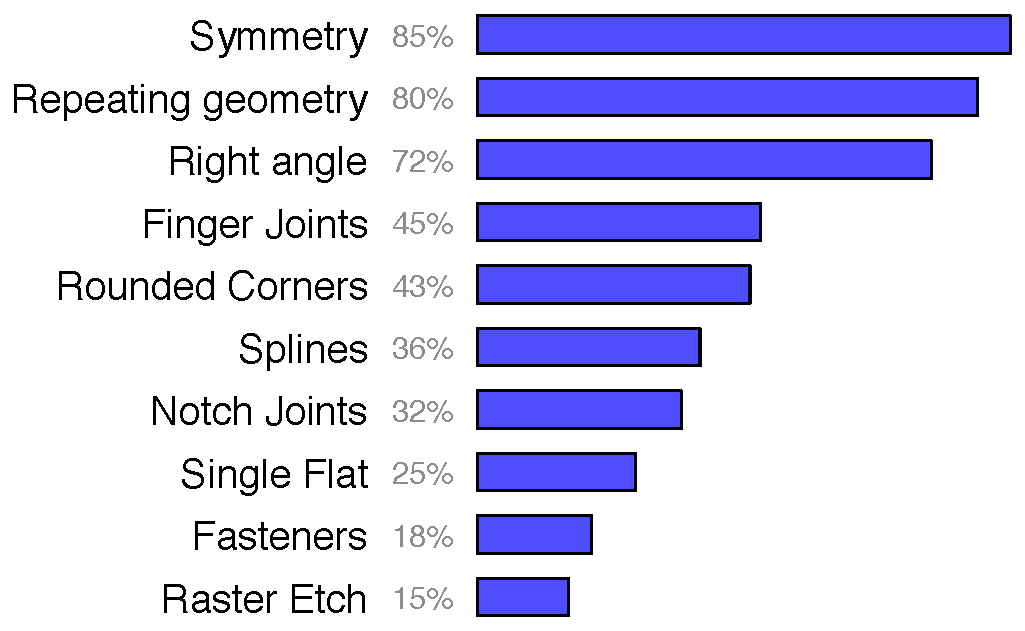
\includegraphics[width=0.6\linewidth]{img/ponoko-graph.pdf}
  \caption[Feature Analysis of Laser Cut Items]{Frequency of features
    of 55 laser-cut designs found on Ponoko and Thingiverse.}
  \label{fig:ponoko}
\end{figure}


We used ten properties to characterize each project, based on our own
experience designing objects for laser cutters, as well as
observations from the formative study. They are:

\begin{itemize}
\item \textit{Symmetry}: Radial/linear symmetry is present.
\item \textit{Repeating geometry}: Line work is repeated several times.
\item \textit{Right Angle}: Edges meet at 90-degree angles.
\item \textit{Notch and Finger Joints}: Two parts come together using one of
  the joints illustrated in Figure~\ref{fig:joint}.
\item \textit{Rounded Corners}: Right-angle corners are slightly blunt.
\item \textit{Splines}: Curved line work (not counting rounded corners).
\item \textit{Single Flat}: The project is composed of a single, flat
  piece of material (e.g. a coaster).
\item \textit{Fasteners}: Use of glue, screws, or bolts.
\item \textit{Raster etch}: Laser cutter etched patterns (e.g. words,
  images) rather than cutting all the way through material.
\end{itemize}

This list of properties helped inform what SIMI should (and should
not) do. 

\begin{figure}[b]
\centering 
\subfloat[Notch joints.] {
  \label{fig:joint-notch} 
  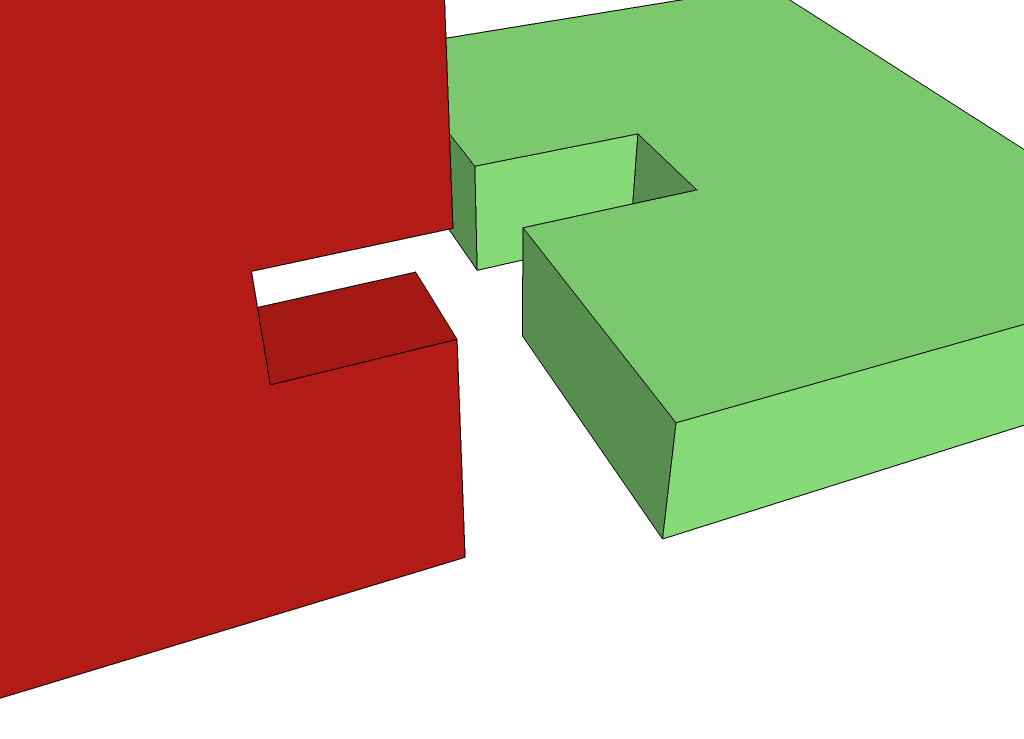
\includegraphics[width=0.3\linewidth]{img/joint-notch.png}
}
\subfloat[Finger (box) joints.] {
    \label{fig:joint-finger}
    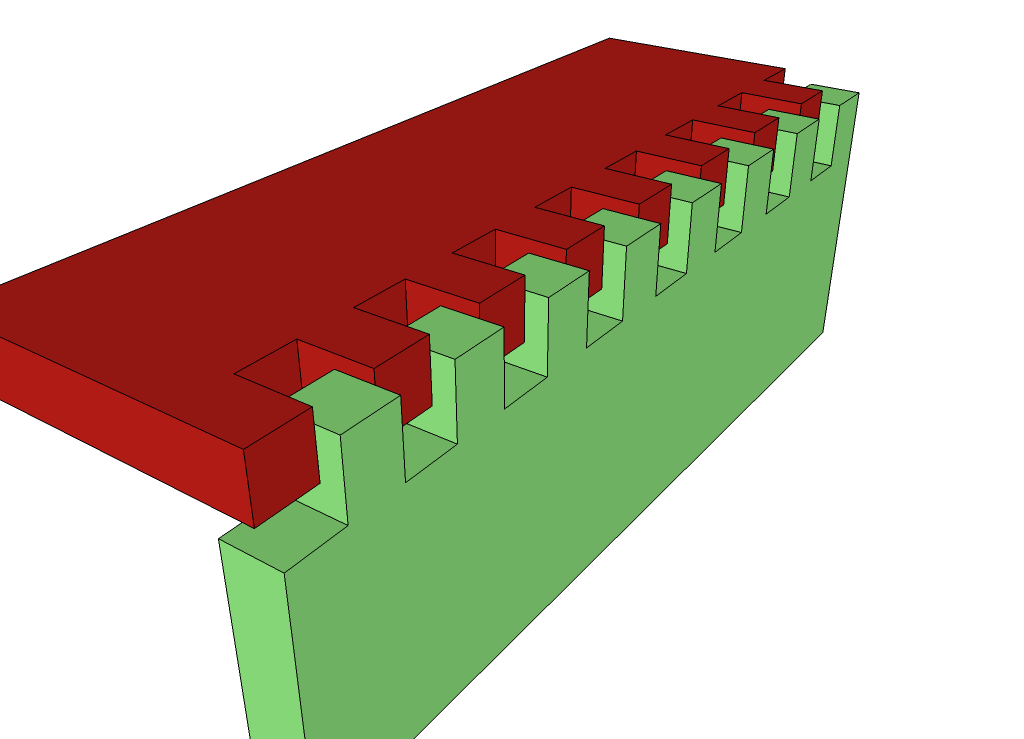
\includegraphics[width=0.3\linewidth]{img/joint-finger.png}
}
\caption[Two common notch types]{Two common methods to join
  parts. Notch joints are used when parts intersect along part
  midsections; finger joints (box joints) join parts along edges.}
\label{fig:joint}
\end{figure}





